\documentclass{article}
\usepackage{graphicx} % Required for inserting images
\usepackage[spanish]{babel}
\usepackage{amsmath}
\usepackage{amsthm}
\usepackage{hyperref}
\usepackage{amssymb}
\usepackage{float}
\usepackage{tikz}
\usepackage{pdfpages}
\usepackage[apa]{biblatex}
\addbibresource{Bibliografía.bib}
\usepackage{pdfpages}
\usepackage{fp}
\usepackage{multicol}
\usepackage{pdflscape}
\usepackage{rotating}

\usepackage[paperwidth=20cm,paperheight=20cm,top=0in,bottom=0in,left=0in,right=0in]{geometry}
\usepackage[dvipsnames]{xcolor}
\usepackage{tikz,pgf}
\usepackage{xintexpr}
\usepackage{appendixnumberbeamer}
\usepackage{booktabs}
\usepackage[scale=2]{ccicons}
\usepackage{pgfplots}
\usepgfplotslibrary{dateplot}
\usepackage{xspace}
\newcommand{\themename}{\textbf{\textsc{metropolis}}\xspace}
\usepackage{pdfpages}
\usepackage{listings}

\definecolor{codegreen}{rgb}{0,0.6,0}
\definecolor{codegray}{rgb}{0.5,0.5,0.5}
\definecolor{codepurple}{rgb}{0.58,0,0.82}
\definecolor{backcolour}{rgb}{0.95,0.95,0.92}

\lstset{
	language=Python,
	basicstyle=\ttfamily,
	keywordstyle=\color{codegreen},
	commentstyle=\color{codegray},
	stringstyle=\color{codepurple},
	numbers=left,
	numberstyle=\tiny\color{codegray},
	breaklines=true,
	breakatwhitespace=true,
	tabsize=4,
	frame=none,
	backgroundcolor=\color{backcolour},
	showstringspaces=false
}

%\usepackage[paperwidth=20cm,paperheight=20cm,top=0in,bottom=0in,left=0in,right=0in]{geometry}
\usepackage[dvipsnames]{xcolor}
\usepackage{tikz,pgf}
\usepackage{xintexpr} %For computing binomial coefficients and their quotients and remainders

\usepackage{geometry}
\geometry{left=1.5in, right=1.5in, top=1.25in, bottom=1.5in}

% Datos del documento
\title{Notas de clase Probabilidad B23}
\author{ Baeza García Cynthia Nayetzi \\
        Jiménez Miranda Luis Antonio  \\
        Elias Vázquez Sergio }
\date{September 2023}

% Inicio del documento
\begin{document}

\begin{titlepage}
    \maketitle
\end{titlepage}

% Índice
\tableofcontents

\clearpage

%---------------------------------------------
%             1. Introducción
%---------------------------------------------
\section{Introducción}

%---------------------------------------------
%         1.1 Tipos de probabilidad
%---------------------------------------------
\subsection{Tipos de probabilidad}
\input{1 Introducción/1.1 Tipos de probabilidad/1.1 Tipos de probabilidad}

\subsubsection{Probabilidad subjetiva}
\noindent La probabilidad subjetiva es aquella que se basa en la experiencia individual. La persona evalúa las posibilidades y asigna los valores de acuerdo a los hechos previos que conoce.

\subsubsection{Probabilidad clásica}
\noindent Sea A un evento para un experimento con un espacio muestral finito $\Omega$. La probabilidad de $A$ es:

\begin{equation}
    P(A) = \frac{n_{A}}{n_{\Omega}}.
    \label{1.1.2 Probabilidad clásica}
\end{equation}

\noindent Donde $n_{A}$ es el número de casos favorables del evento A y $n_{\Omega}$ es el número de elementos del espacio muestral. \\

\noindent\underline{Nota:} Cada evento del espacio muestral tiene la misma probabilidad de ocurrir.\\

\noindent\textbf{Ejemplo: } Si se desea calcular la probabilidad de que al tirar un dado salga un número par, el espacio muestral sería 

\begin{equation*}
    \Omega = \{1,2,3,4,5,6\},
\end{equation*}

\noindent por lo que $n_{\Omega} = 6$ y $n_{A = \{2,4,6\}} = 3$, por lo tanto

\begin{equation*}
    P(A) = \frac{3}{6} = \frac{1}{2}
\end{equation*}

\subsubsection{Probabilidad frecuentista}
\noindent La probabilidad frecuentista se refiere a qué tan probable resulta un suceso si un experimento se repite muchas veces.

\begin{equation}
    P(A) = \frac{n(A)}{n}
    \label{1.1.2 Probabilidad frecuentista}
\end{equation}

\noindent\textbf{Ejemplo: } Supongamos que se ha lanzado un moneda diez veces, de tal manera que en tres ocasiones ha salido águila, y siete veces ha salido sol. Entonces la probabilidad frecuentista de que haya salido ágila es

\begin{equation*}
    P(A_{\text{Águila}}) = \frac{3}{10}
\end{equation*}

\noindent mientras que la probabilidad para el caso en el que salió sol es

\begin{equation*}
    P(A_{\text{Sol}}) = \frac{7}{10}.
\end{equation*}

\subsubsection{Probabilidad geométrica}
\noindent Se basa en conjuntos geométricos, áreas y subconjuntos en un espacio acotado, donde a cada subconjunto de $\Omega$ con área bien definida, se le asigna una probabilidad que es la proporción entre su área y el área de $\Omega$.

\begin{equation}
    P(A) = \frac{\text{Área de A}}{\text{Área de $\Omega$}} 
\end{equation}
\\
\noindent\textbf{Ejemplo:} Imagina que vas a tomar un autobús. El autobús llaga entre las 12 pm y la 1 pm. Es decir, los tiempos de llegada tuyo y del autobús son valores $x \in [0, 60]$. Además, supongamos que cuando el autobús llega, permanece en la parada 5 minutos antes de irse; y cuando tú llegas, esperas 20 minutos antes de irte si el autobús no llega. ¿Cuál es la probabilidad de que tomes el autobús? \\

\noindent\textbf{Solución:} En este caso podemos considerar nuestro espacio muestral de la siguiente manera

\begin{equation*}
    \Omega = [0,60] \times [0,60] = \{(x,y) \in \mathbb{R}^{2} | x \in [0,60] \wedge y \in [0,60]\}
\end{equation*}

\begin{figure}[H] 
    \centering 
    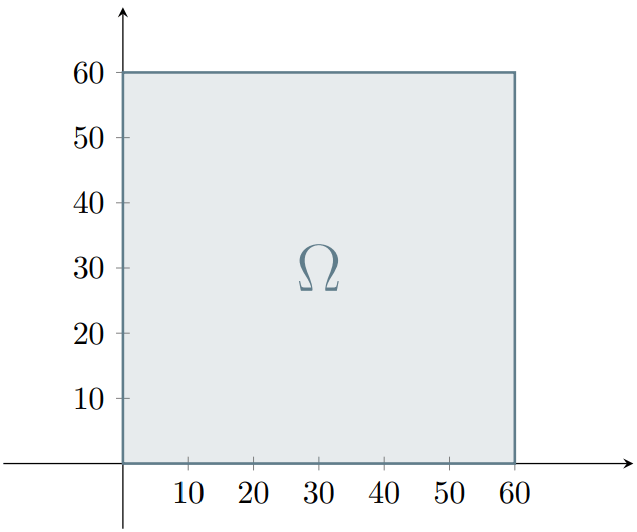
\includegraphics[width=0.4\textwidth]{1 Introducción/1.1 Tipos de probabilidad/1.1 Imágenes/Probabilidad geometrica 2.png}
    \caption{Espacio muestral $\Omega$}
\end{figure}

\noindent Ahora, como el autobús se espera 5 minutos después de llegar, tu tiempo de llegada $x$ debe ser menor o igual a $y+5$, es decir, $a \leq y+5$. Podemos tomar a este evento como el evento $A$ y se representaría de la siguiente manera

\begin{equation*}
    A = \{(x,y) \in \Omega | x-5 \leq y\}
\end{equation*}

\begin{figure}[H] 
    \centering 
    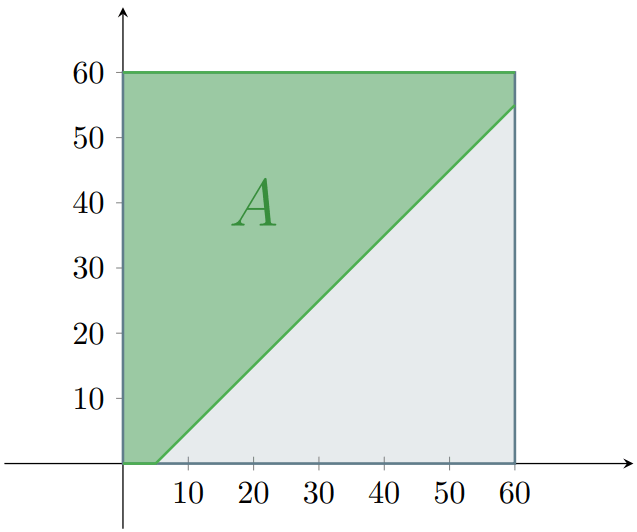
\includegraphics[width=0.4\textwidth]{1 Introducción/1.1 Tipos de probabilidad/1.1 Imágenes/Probabilidad geometrica 3.png}
    \caption{Evento $A$}
\end{figure}

\noindent Por otra parte, tu esperas el autobús por 20 minutos, por lo que $x \geq y-20$, entonces

\begin{equation*}
    B = \{(x,y) \in \Omega | y \leq x+20\}
\end{equation*}

\begin{figure}[H] 
    \centering 
    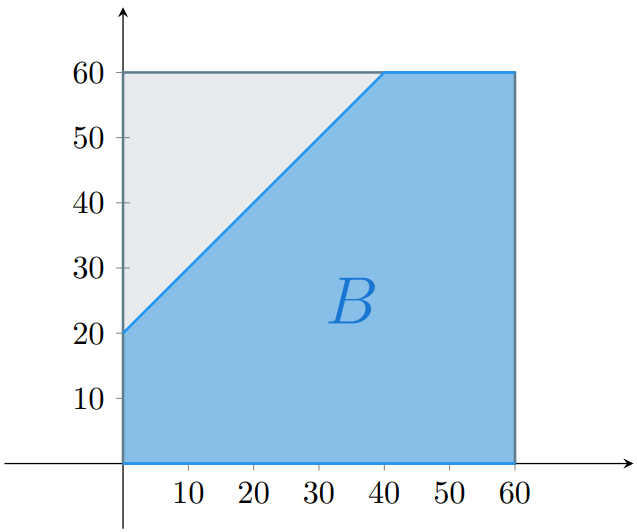
\includegraphics[width=0.4\textwidth]{1 Introducción/1.1 Tipos de probabilidad/1.1 Imágenes/Probabilidad geometrica 4.png}
    \caption{Evento $B$}
\end{figure}

\noindent La intersección de ambas regiones representa cuando tú y el autobús coinciden.

\begin{figure}[H] 
    \centering 
    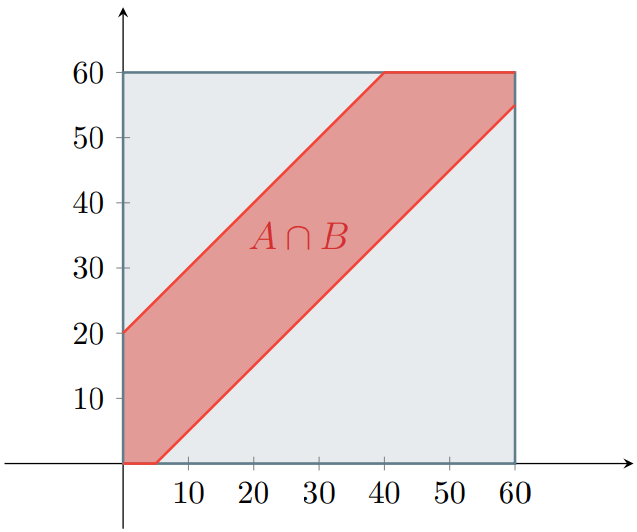
\includegraphics[width=0.4\textwidth]{1 Introducción/1.1 Tipos de probabilidad/1.1 Imágenes/Probabilidad geometrica 5.png}
    \caption{$A \cap B$}
\end{figure}

\noindent Notemos que gráficamente $(A \cap B)^{c}$ forma dos triangulos de área $40^{2}/2$ y $55^{2}/2$

\begin{figure}[H] 
    \centering 
    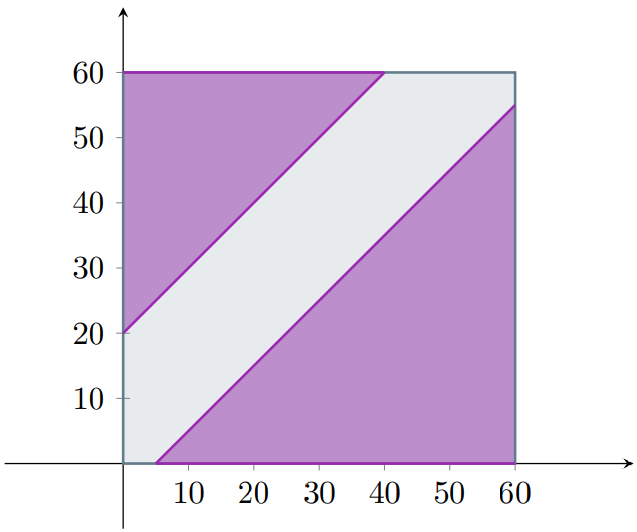
\includegraphics[width=0.4\textwidth]{1 Introducción/1.1 Tipos de probabilidad/1.1 Imágenes/Probabilidad geometrica 6.png}
    \caption{Evento $A$}
\end{figure}

Por lo que podemos calcular la probabilidad de $A \cap B$ como:

\begin{equation*}
    \begin{split}
        P(A \cap B) & = P(\Omega) - P((A \cap B)^{c}) \\
        & = 1 - \left(\frac{\frac{40^{2}}{2}+\frac{55^{2}}{2}}{60^{2}}\right) \\
        & = 1- \frac{4625}{7200} \\
        & = \frac{103}{288}
    \end{split}
\end{equation*}


\subsubsection{Probabilidad axiomática}
\noindent Dado un experimento y un espacio muestral $\Omega$, se asigna a cada evento $A$ un número $P(A)$, que debe satisfacer los axiomas siguientes: \\

\noindent\textbf{Axioma 1:} Para cualquier evento $A$
\begin{equation*}
    0 \leq P(A)
\end{equation*}

\noindent\textbf{Axioma 2:} 
\begin{equation*}
    P(\Omega) = 1
\end{equation*}

\noindent\textbf{Axioma 3:} Si $A_{1}, A_{2}, ...$ es un conjunto de eventos mutuamente excluyentes, entonces:
\begin{equation*}
    P(A_{1} \cup A_{2} \cup ...) = \sum_{i = 1}^{\infty} P(A_{i})
\end{equation*}




%---------------------------------------------
%         1.2 Teoría de Conjuntos
%---------------------------------------------
\clearpage
\subsection{Teoría de conjuntos}
\noindent \textbf{Definici\'on.} \\
    Un conjunto puede definirse como una lista o colección bien definida de objetos; los objetos comprendidos en un conjunto son llamados sus ‘elementos o miembros’. \\

\noindent    \textbf{Ejemplos:}
    \begin{itemize}
        \item Los n\'umeros $1, 3, 7$ y $10$,
        \item Los estudiantes del CIC, 
        \item Los r\'ios de M\'exico,
        \item Los n\'umeros pares enteros: $0, 2, 4, 6...$
    \end{itemize}

\noindent    \textbf{Notaci\'on.} \\ 
\noindent     Un conjunto puede ser denotado con letras may\'usculas, como por ejemplo,
     \begin{center}
         $A, B, C, X, Y, ...$
     \end{center}
 
\noindent     Mientras que las letras min\'usculas se utilizan para indicar sus elementos.
     \begin{center}
         $a,b,c,x,y,z, ...$
     \end{center}

\noindent  Existen dos formas de especificar un conjunto: \\ 
    
    \begin{itemize}{}
        \item  \textbf{M\'etodo de extensi\'on:} Que consiste en listar sus elementos.
        \item \textbf{M\'etodo de comprensi\'on:} Describir alguna propiedad conservada por todos los miembros del conjunto.\\ 
    \end{itemize}

   
    \begin{center}
        \begin{tcolorbox}
        \textbf{Ejemplo: } El conjunto de las vocales del alfabeto.      \vspace{5px}
            \begin{itemize}
                \item $ V = \lbrace a, e, i, o, u \rbrace $ \hspace{2.35cm} \textbf{M\'etodo de extensi\'on } 
                \item $ V =\lbrace x \mid x $ es una vocal $\rbrace$  \hspace{1cm} \textbf{M\'etodo de comprensi\'on} \\ \vspace{2px}
                 Léase \textit{“El conjunto de los elementos x tal que x es una vocal”.}
            \end{itemize}
        \end{tcolorbox} 
    \end{center} 

\subsubsection{Conjunto universo y conjunto vacío.}

\noindent   \textbf{Conjunto universo.} \\
\noindent     Todos los conjuntos están contenidos en algún gran conjunto fijo, llamado \textbf{conjunto universal o universo}. Denotado por:
    \begin{center}
        $U$,
    \end{center}
\noindent     a menos que se especifique lo contrario.\\ \vspace{6px}
    
\noindent \textbf{Conjunto vac\'io.} \\
\noindent     Tambi\'en llamado \textbf{conjunto nulo}. Es aquel que no contiene elementos en él, se denota como, 
    \begin{center}
        $\emptyset$ \hspace{0.5cm} \'o \hspace{0.5cm} $\lbrace \rbrace$.
    \end{center}
\noindent     \'Este es subconjunto de cualquier otro conjunto. 

\subsubsection{Subconjuntos}
\noindent Si cada elemento de un conjunto $A$ es también un elemento de un conjunto $B$, entonces $A$ se le llama \textbf{subconjunto} de $B$. También decimos que $A$ está contenido en $B$ o $B$ contiene a $A$. Esta relación se escribe:

    \begin{equation}
            A \subseteq B  \hspace{0.5cm} \text{\'o} \hspace{0.5cm} B \supseteq A
    \end{equation}

\noindent     si $A$ no es un subconjunto de $B$, es decir, si al menos un elemento de $A$ no pertenece a $B$, escribimos:

    \begin{equation}
            A \nsubseteq B  \hspace{0.5cm}  \text{\'o} \hspace{0.5cm} B \nsupseteq A
    \end{equation}


\noindent \textbf{Conjutos disjuntos.} \\
\noindent     Dos conjuntos $A$ y $B$ son disjuntos si no tienen ning\'un elemento en com\'un, tales que  $A \cap B = \emptyset$. \\
\noindent \textbf{Por ejemplo:}
    \begin{center}
         $A = \lbrace 1, 3\rbrace $\hspace{0.5cm}  $B = \lbrace 1, 2, 3\rbrace$  \hspace{0.5cm}  $C = \lbrace  2\rbrace$
    \end{center}
   
    $A$ y $C$ son conjuntos disjuntos.

\subsubsection{Diagramas de Venn}
\noindent  Es una representaci\'on pict\'orica de conjuntos donde los conjuntos est\'an representados por \'areas cerradas en el plano.
    \begin{center}
        \begin{tikzpicture}
                % Conjunto universal
                \draw[fill=white!20] (-1.5,-1.5) rectangle (3,1.5) node[above] {$U$};
                                     
                % Conjunto B
                \draw[fill=gray!30] (1.7,0.75) circle (0.5cm) node[above] {$B$};
                % Conjunto A
                \draw[fill=gray!30] (0,0) circle (1cm) node[above] {$A$};
                % Título
                \node at (0.8,-2) {A y B conjuntos disjuntos.};
            \end{tikzpicture}
    \end{center}\clearpage

\subsubsection{Operaciones con conjuntos}

\noindent  \textbf{Uni\'on de conjuntos.}\\
\noindent   Denotada como $A \cup B$, son todos los elementos  que pertenecen a $A$ y a $B$.
    
            \begin{center}
                $A \cup B = \lbrace x : x \in A \hspace{0.1cm} \lor \hspace{0.1cm} x \in B\rbrace$
            \end{center}

    \begin{center}
            \begin{tikzpicture}
                 % Conjunto universal
                \draw[fill=white!20] (-1.5,-1.5) rectangle (3,1.5) node[above] {$U$};
                                         
                 % Conjunto B
                \draw[fill=gray!30] (1.5,0) circle (1cm) node[above] {$B$};
                
                % Conjunto A
                \draw[fill=gray!30] (0,0) circle (1cm) node[above] {$A$};
    
                % Título
                \node at (1,-2) {Uni\'on de $A$ con $B$.};
            \end{tikzpicture}
    \end{center}

\noindent \textbf{Intersección de conjuntos.}\\
\noindent  Hace referencia a todos los elementos que pertenecen tanto a $A$ como a $B$ se denota como $A \cap B$ donde,

            \begin{center}
                $A \cup B = \lbrace x : x \in A \hspace{0.1cm} \land \hspace{0.1cm} x \in B\rbrace$
            \end{center}      
        
    \begin{center}
        \begin{tikzpicture}  
            % Conjunto universal
            \draw[fill=white!20] (-1.5,-1.5) rectangle (3,1.5) node[above] {$U$};
             % Conjunto A
            \draw[fill=white!30] (0,0) circle (1cm) node[above] {$A$};
            % Conjunto B
            \draw[fill=white!30] (1.5,0) circle (1cm) node[above] {$B$};

            % Intersección de conjuntos
            \begin{scope}
            \clip (0,0) circle (1cm);
            \clip (1.5,0) circle (1cm);
            \fill[gray!30] (-2,-2) rectangle (4,2);
            \end{scope}
                   
            % Título
            \node at (1,-2) {Intersección de $A$ con $B$.};
        \end{tikzpicture}
     \end{center}


\noindent  \textbf{Complemento.} \\
\noindent El \textbf{complemento absoluto}, o simplemente \textbf{complemento de un conjunto} $A$, denotado por  $A^{c}$, es el conjunto de elementos que pertenecen al conjunto universo $U$ mas no al conjunto $A$.
    
    \begin{center}
            $A^{c} = \lbrace x : x \in U,  x \notin A\rbrace$
        
            \begin{tikzpicture}                  
                % Conjunto universal
                \draw[fill=gray!20] (-1.5,-1.5) rectangle (3,1.5) node[above] {$U$};
    
                % Complemento de A
                \begin{scope}
                    \clip (0,0) circle (1cm);
                    \fill[white, opacity=0.1] (-2,-2) rectangle (2,2);
                \end{scope}
                        
                % Conjunto B
                \draw[fill=gray!20] (1.5,0) circle (1cm) node[above] {$B$};
                % Conjunto A
                \draw[fill=white!30] (0,0) circle (1cm) node[above] {$A$};
             
                % Título
                \node at (1,-2) {Complemento de A.};
            \end{tikzpicture} 
    \end{center}


\noindent \textbf{Diferencia y Diferencia sim\'etrica.}\\
\noindent La \textbf{diferencia} entre $A$ y $B$, es denotada por $A\setminus B$, es el conjunto de elementos que pertenecen a $A$ mas no pertenecen a $B$, es decir:
    
    \begin{center}
            $A \setminus  B = \lbrace x : x \in A  \hspace{0.1cm} \lor \hspace{0.1cm} x \notin B\rbrace$
            
    
            \begin{tikzpicture}
                 % Conjunto universal
                \draw[fill=white!20] (-1.5,-1.5) rectangle (3,1.5) node[above] {$U$};

                % Conjunto A
                \draw[fill=gray!30] (0,0) circle (1cm) node[above] {$A$};
                
                 % Conjunto B
                \draw[fill=white!30] (1.5,0) circle (1cm) node[above] {$B$};
                
    
                % Título
                \node at (1,-2) {Diferencia $A \setminus B$.};
            \end{tikzpicture}

    \end{center}

\noindent \textbf{Diferencia y Diferencia sim\'etrica.}\\
\noindent  La \textbf{diferencia sim\'etrica} de dos conjutnos $A$ y $B$, denotada como $A \oplus B$, consiste en los elementos que pertenecen a $A$ \'o a $B$ mas no a los elementos que pertenecen a ambos $A$ y $B$, esto es:

        \begin{center}
            $A \oplus B = (A \cup B)\setminus(A \cap B)$ \hspace{1cm} \'o \hspace{1cm} $A \oplus B = (A \setminus B)\cup (B^{'} \setminus A)$\vspace{15px} \\
              

            \begin{tikzpicture}  
            % Conjunto universal
            \draw[fill=white!20] (-1.5,-1.5) rectangle (3,1.5) node[above] {$U$};
             % Conjunto A
            \draw[fill=gray!30] (0,0) circle (1cm) node[above] {$A$};
            % Conjunto B
            \draw[fill=gray!30] (1.5,0) circle (1cm) node[above] {$B$};

            % Intersección de conjuntos
            \begin{scope}
            \clip (0,0) circle (1cm);
            \clip (1.5,0) circle (1cm);
            \fill[white!30] (-2,-2) rectangle (4,2);
            \end{scope}
                   
            % Título
            \node at (1,-2) {Diferencia sim\'etrica $A \oplus B$.};
            \end{tikzpicture}
    \end{center}

\subsubsection{Clases de conjuntos}

\noindent    Si se desea considerar algunos de los conjuntos de una clase determinada de conjuntos, se utiliza el término \textbf{subclase} o \textbf{subcolecci\'on}.\\

    \textbf{Ejemplos:}
    \begin{itemize}
         \item  En un conjunto de líneas cada línea es un conjunto de puntos. 
        \item  Los miembros de la clase $\lbrace \mid2,3\mid, \mid2\mid, \mid5,6\mid\rbrace$ son los conjuntos $\mid2,3\mid, \mid2\mid y \mid5,6\mid.$
    \end{itemize}

\subsubsection{Teoremas relativos a conjuntos}
\noindent  A continuaci\'on se listan algunas leyes de \'algebra de conjuntos en los siguientes cuadros.\\

\begin{table}[ht]
    \centering
    \renewcommand{\arraystretch}{1.5} % Aumentar la altura de las filas de la tabla
    \begin{tabular}{|p{6cm}|p{5cm}|}
        \hline
        \textbf{Ley} & \textbf{Expresión} \\
        \hline
        Ley conmutativa de la unión  & $A \cup B =  B \cup A$ \\
        \hline
       Ley asociativa de la unión &  $A \cup (B \cap C) = (A \cup B)  \cup C$ \\
        \hline
        Ley conmutativa de la intersección & $A \cap B =  B \cap A$ \\
        \hline
        Ley asociativa de la intersección & $A \cap (B \cup C) = (A \cap B) \cap C$ \\
        \hline
        Ley de la Anulación & $A \cap \varnothing = \varnothing$ \hspace{1cm}  $A \cup U = U$ \\
        \hline
        
        
    \end{tabular}
    \caption{Leyes del Álgebra de Conjuntos (Parte 1).}
\end{table}

\begin{table}[ht]
        \centering
        \renewcommand{\arraystretch}{1.5} % Aumentar la altura de las filas de la tabla
        \begin{tabular}{|p{6cm}|p{5cm}|}
            \hline
            \textbf{Ley} & \textbf{Expresión} \\
            \hline
            Ley de la Complemento Universal & $A \cap U' = \varnothing$ \hspace{1cm} $A \cup \varnothing' = U$ \\
            \hline
            Primera ley distributiva & $A \cap (B \cup C) = (A \cap B) \cup (A \cap C)$ \\
            \hline

             Segunda ley distributiva &  $A \cup (B \cap C) = (A \cup B) \cap (A \cup C)$ \\
            \hline
            
            Ley de De Morgan & $(A \cap B)' = A' \cup B'$ \newline$(A \cup B)' = A' \cap B'$ \\
            \hline
            Ley del Complemento de la Intersección & $(A \cap B)' = A' \cup B'$ \\
            \hline
            Ley del Complemento de la Unión & $(A \cup B)' = A' \cap B'$ \\
            \hline
        \end{tabular}
        \caption{Leyes del Álgebra de Conjuntos (Parte 2).}
        \label{tabla:leyes-conjuntos}
    \end{table}


%---------------------------------------------
%         1.3 Relaciones 
%---------------------------------------------
% Esto es parte de lo que expuse en conjuntos pero como era varia cosa
% lo puse aparte para acomodarlo mejor. Besitos uwu
\clearpage
\subsection{Relaciones}
 \noindent \textbf{Definición.} \\
 \noindent  Sea $A$ y $B$ conjuntos, una \textbf{relación binaria}, o simplemente, una relación de $A$ a $B$, es un subconjunto de $A \times B$. Supongamos que $R$ es una relación de $A$ a $B$. Entonces $R$ es un conjunto de pares ordenados donde cada primer elemento proviene de $A$ y cada segundo elemento proviene de $B$. \\
    

 \noindent  El \textbf{\textit{dominio}} de una relación $R$ de $A$ a $B$ es el conjunto de todos los primeros elementos de los pares ordenados que pertenecen a $R$, por lo que es un subconjunto de $A$; y el rango de $R$ es el conjunto de todos los segundos elementos, por lo que es un subconjunto de $B$. \\





 

\subsubsection{Relaciones universales y relaciones vacías}

    
\noindent    Sea $A$ cualquier conjunto, entonces $A \times A$ y $\varnothing$ son subconjuntos de $A \times A$ y, por tanto, son relaciones en $A$ llamadas \textit{relación universal} y \textit{relación vacía}, respectivamente. Por tanto, para cualquier relación $R$ sobre $A$, tenemos que:
\[
\varnothing \subseteq R \subseteq A \times A
\]

\subsubsection{Relación inversa}

 \noindent      Sea $R$ cualquier relación de un conjunto $A$ a un conjunto $B$. La inversa de $R$, denotada por $R^{-1}$, es la relación de $B$ a $A$ que consta de aquellos pares ordenados que, invertidos, pertenecen a $R$; es decir,
    \[
    R^{-1} = \{(b, a) : (a, b) \in R\}
    \]
    
 \noindent     \textbf{Por ejemplo,} si $R = \{(1, y), (1, z), (3, y)\}$, entonces $R^{-1} = \{(y, 1), (z, 1), (y, 3)\}$.

\subsubsection{Representación en conjuntos finitos}

    
 \noindent   Formas de representar una relación $R$ de $A$ a $B$.  \\
 
 \noindent \textbf{Por ejemplo,} si $R$ es una relación de $A = \{1, 2, 3\}$ a $B = \{x, y, z\}$, y $R = \{(1, y), (1, z), (3, y)\}$. \\
    

    \noindent \textbf{ Matriz de la relación.}\\
    \noindent         Formar un arreglo rectangular cuyas filas estén etiquetadas por los elementos de $A$ y cuyas columnas estén etiquetadas por los elementos de $B$. Poner un $1$ o $0$ en cada posición del arreglo según si $a \in A$ está o no relacionada con $b \in B$.

                
                \[
                \begin{bmatrix}
                    & x & y & z \\
                  1 & 0 & 1 & 1 \\
                  2 & 0 & 0 & 0 \\
                  3 & 0 & 1 & 0 \\
                \end{bmatrix}
                \]

    \vspace{10px}
    \noindent \textbf{Diagrama de flechas de la relación}.\\
             Escribir los elementos de $A$ y los elementos de $B$ en dos conjuntos disjuntos, y luego dibujar una flecha desde $a \in A$ hasta $b \in B$ siempre que $a$ esté relacionado con $b$. 

\subsubsection{Tipos de relaciones}
 \noindent  Considere el conjunto $A$ dado.

 \begin{itemize}
    \item \textbf{Relaciones Reflexivas}: Una relación $R$ en el conjunto $A$ es reflexiva si $a$ $R$ $a$ para cada $a \in A$, es decir, si $(a, a) \in R$ donde $a \in A$. Por tanto, $R$ no es reflexiva si existe un $a \in A$ tal que $(a, a) \notin R$.\\


    \item  \textbf{Relaciones Simétricas}: Una relación $R$ en un conjunto $A$ es simétrica si siempre que $a$ $R$ $b$, entonces $b$ $R$ $a$, es decir, si siempre que $(a, b) \in R$, entonces $(b, a) \in R$. Por tanto, $R$ no es simétrica si existe $a, b \in A$ tal que $(a, b) \in R$ pero $(b, a) \notin R$. \\

    \item \textbf{Relaciones Antisimétricas}: Una relación $R$ en un conjunto $A$ es antisimétrica si siempre que $a$ $R$ $b$ y $b$ $R$ $a$, entonces $a = b$, es decir, si siempre que $(a, b)$ y $(b, a)$ pertenecen a $R$, entonces $a = b$. Por tanto, $R$ no es antisimétrica si existe $a, b \in A$ tal que $(a, b)$ y $(b, a)$ pertenecen a $R$, pero $a$ es diferente de $b$. \\

    \item    \textbf{Relaciones Transitivas}: Una relación $R$ en un conjunto $A$ es transitiva si siempre que $a$ $R$ $b$ y $b$ $R$ $c$, entonces $a$ $R$ $c$, es decir, si siempre que $(a, b), (b, c) \in R$, entonces $(a, c) \in R$. Así que $R$ no es transitiva si existe $a, b, c \in A$ tal que $(a, b), (b, c) \in R$, pero $(a, c) \notin R$. \\
\end{itemize}

\subsubsection{Funciones}

\noindent \textbf{Definición.}
\noindent Una función $f: A \to B$ es una relación de $A$ a $B$ (es decir, un subconjunto de $A \times B$) tal que para cada $a \in A$, pertenece a un único par ordenado $(a, b)$ en $f$.

Toda función dada como la relación del conjunto A al conjunto B ($f: A \to B$), es llamado como el grafo de $f$ y definido como:

\begingroup
    \centering $f = \lbrace(a,b) : a \in A, b = f(a)\rbrace$
\endgroup 

%---------------------------------------------
%       Tareas Capítulo 1: Introducción
%---------------------------------------------

\clearpage
\subsection{Tareas Capítulo 1}

\subsubsection{Experimentos deterministas y aleatorios}
\noindent \textbf{Experimento determinista}: Un experimento determinista es aquel que tiene un resultado predecible y reproducible siempre que se mantengan las mismas condiciones y parámetros iniciales. \\

\noindent \textbf{Ejemplos de expermientos deterministas}

\begin{itemize}
    \item Medir la longitud de una mesa.

    \item Calcular el área de un círculo.

    \item Sumar de dos números enteros

    \item Encender una bombilla con el interruptor

    \item Hervir agua a $100 ^{o}C$ 

    \item Medir la velocidad de una pelota deslizándose por una pendiente desde la misma altura.

    \item Medir la velocidad al disparar una bala.

    \item Medir la velocidad de un objeto que cae desde una ventana.

    \item Juntar un imán con un metal.

    \item Medir la corriente eléctrica de un circuito.
\end{itemize}

\noindent \textbf{Experimento aleatorio}: Un experimento aleatorio es aquel en el que si lo repetimos con las mismas condiciones iniciales no garantiza los mismos resultados. \\

\noindent \textbf{Ejemplos de expermientos aleatorios}

\begin{itemize}
    \item Lanzar una moneda y observar si sale cara o cruz. 

    \item Extraer una carta de una baraja y ver su palo y número. 

    \item Tirar un dado y ver el número que aparece en la cara superior. 

    \item Elegir una persona al azar de un grupo y preguntarle su edad. 

    \item Comprar un boleto de lotería y ver si resulta premiado.

    \item Medir el spin de un electrón.

    \item Escoger una bola de un saco.

    \item Elegir las fichas de domino.

    \item Apostar a un número en la ruleta.

    \item Desarmar un cubo de rubik sin un orden.
\end{itemize}

\subsubsection{Triángulo de Pascal}
%Triangulo de pascal
\newlength{\R}
\setlength{\R}{.75cm}
\newcommand\mycolor{white}

%% https://tex.stackexchange.com/questions/34424/how-do-i-calculate-n-modulo-3-in-latex/34425#34425
\newcommand{\modulo}[2]{%
  \FPeval{\result}{trunc(#1-(#2*trunc(#1/#2,0)),0)}\result%
}

%%  #1 determines which hexagons are filled (default is 2); #2 is number of rows

\newcommand{\makesierp}[2][2]{%
    \begin{tikzpicture}[line width=.8pt]
        \foreach \k in {0,...,#2}{
            \begin{scope}[shift={(-60:{sqrt(3)*\R*\k})}]
                \pgfmathtruncatemacro\ystart{#2-\k}
                \foreach \n in {0,...,\ystart}{
                    \pgfmathtruncatemacro\newn{\n+\k}
                    \pgfmathsetmacro{\myvalue}{1}
                    \ifnum\k>0
                        \foreach \b in {1,...,\k}{
                            \FPeval\myvalue{trunc(\myvalue*(\newn-\b+1)/\b:0)}
                            \global\let\myvalue=\myvalue
                        }
                    \fi
                    \modulo{\myvalue}{#1}%
                    \ifnum\result=0 \def\mycolor{green}\fi%
                    \begin{scope}[shift={(-120:{sqrt(3)*\R*\n})}]
                        \draw[fill=\mycolor!20] 
                        (30:\R) \foreach \x in {90,150,...,330} {
                        -- (\x:\R)}
                        --cycle (90:0)node[font=\tiny] {$\mathbf{\myvalue}$};
                    \end{scope}
                }
            \end{scope}
        }
    \end{tikzpicture}
}

\textbf{Definition of Pascal's Triangle} \\
Pascal's Triangle is a mathematical construct that is used in various areas of mathematics, particularly in combinatorics and algebra. It is a triangular array of numbers in which each number is the sum of the two numbers directly above it. The triangle is named after the French mathematician Blaise Pascal, who studied its properties in the 17th century, although it was known to Chinese mathematicians over 500 years earlier.  \\

Pascal's Triangle is an infinite triangular array of numbers in which the first and last numbers in each row are always 1, and each of the interior numbers is the sum of the two numbers directly above it.  \\

%Triangulo de pascal
\resizebox{0.8\textwidth}{!}{ 
    \makesierp{20}
}
 %INSERTAR

\vspace{1cm}
\noindent \textbf{Applications of Pascal Triangle}
Pascal's Triangle, a mathematical construct developed by Blaise Pascal, has several applications in the field of biology. Here are some of the uses of Pascal's Triangle in biology:  \\

\noindent 1. Genetic Inheritance: Pascal's Triangle can be used to understand and calculate the probabilities of different genetic inheritance patterns. For example, it can help determine the probability of specific genotypes or phenotypes in offspring when considering traits governed by multiple alleles or multiple genes. \\

\noindent 2. Population Genetics: In the study of population genetics, Pascal's Triangle can be employed to model changes in allele frequencies over time. It aids in predicting the distribution of genotypes within a population across generations, considering factors like genetic drift, mutation rates, and selection pressures. \\

\noindent 3. Probability in Genetics: Pascal's Triangle is useful for calculating probabilities in genetic crosses involving complex inheritance patterns. It can help determine the likelihood of certain genetic outcomes in offspring, which is essential for understanding the genetic basis of traits and diseases. \\

\noindent 4. Microbial Population Growth: In microbiology, Pascal's Triangle can be applied to model the growth of microbial populations. It helps researchers predict population sizes over time under various conditions, such as different growth rates and mutation rates. \\

\noindent 5. Evolutionary Biology: Pascal's Triangle can be used to analyze the probabilities of specific genetic changes occurring over time within populations. This is crucial for studying the emergence of new traits and adaptations during evolution. \\

\noindent 6. Phylogenetics: In phylogenetics, which focuses on the evolutionary relationships among species, Pascal's Triangle can be used to calculate the probabilities of different phylogenetic tree topologies based on genetic data. It aids in inferring the evolutionary history and relationships of species. \\

\noindent 7. Population Ecology: Pascal's Triangle can be employed in population ecology to model changes in population size over time. It helps predict how populations of different species interact within ecological communities and how they respond to changes in birth rates, death rates, immigration, and emigration. \\

\noindent 8. Epidemiology: In epidemiology, Pascal's Triangle can be used to model the spread of diseases within populations. It aids in understanding the probabilities of individuals becoming infected, recovering from infections, or transmitting diseases to others. This is valuable for disease control and public health efforts. \\

\noindent 9. Genetic Mapping: Pascal's Triangle can assist in genetic mapping by           calculating probabilities related to the linkage of genetic markers on chromosomes. It helps determine the likelihood of two or more genes segregating together or independently during meiosis. \\

\noindent 10. Probability of Mutations: Researchers can use Pascal's Triangle to calculate the probabilities of specific types of mutations occurring in DNA sequences. This is crucial for understanding the molecular basis of genetic diseases and evolutionary processes. \\

\textbf{Example: GENETICS}

Pascal's Triangle and Risk Calculations \\
Introduction: \\
Pascal's Triangle, based upon the French Mathematician Blaise Pascal, is used in genetic counselling to calculate the probability of obtaining a particular number or distribution of events of one kind knowing the probability of each event occurring independently. This is a simpler approach to the use of the Binomial Distribution. \\

Principles: Pascal's Triangle \\
The simplest way to look at the role of Pascal's Triangle is to study a family with an autosomally inherited disorder. \\
What are Autosomes? \\
Autosomes are non-sex chromosomes found in the cells of an organism. In humans and many other organisms, autosomes make up the majority of an individual's total chromosome number. They are distinct from the sex chromosomes (X and Y in humans) that determine an individual's sex. Autosomes carry genes responsible for various traits and characteristics unrelated to sexual development.
Consider the following scenario: \\
A 45-year-old man is diagnosed with Type 1 Antithrombin deficiency and is concerned that he may have passed it onto his three children. His partner has normal functional Antithrombin levels. what are the risk that his children will have Type 1 Antithrombin deficiency. \\
Antithrombin deficiency is inherited as an autosomal dominant disorder. \\

\textbf{Example: GENETICS}
The Family Pedigree is shown below: \\

\begin{figure}
    \centering
    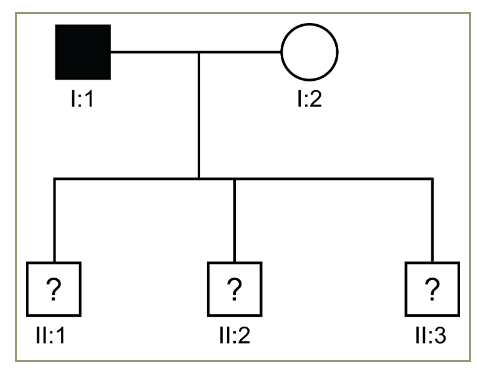
\includegraphics[width=0.5\linewidth]{1 Introducción/Tareas Capítulo 1/Triángulo de Pascal/Picture2.png}
    \caption{Example: GENETICS}
    \label{fig:enter-label}
\end{figure}

\textbf{What are the Risks?} \\
1. All 3 of his children [II:1, II:2 and II:3] will have Type 1 Antithrombin deficiency? \\

2. All 3 of his children [II:1, II:2 and II:3] will not have Type 1 Antithrombin deficiency? \\

3. 1 of his children will have Type 1 Antithrombin deficiency? \\

4. 2 of his children will have Type 1 Antithrombin deficiency? \\

We can derive the answers for these questions using Pascal's Triangle - derived by expanding (p +q)n. This is shown diagrammatically below: \\

\begin{figure}
    \centering
    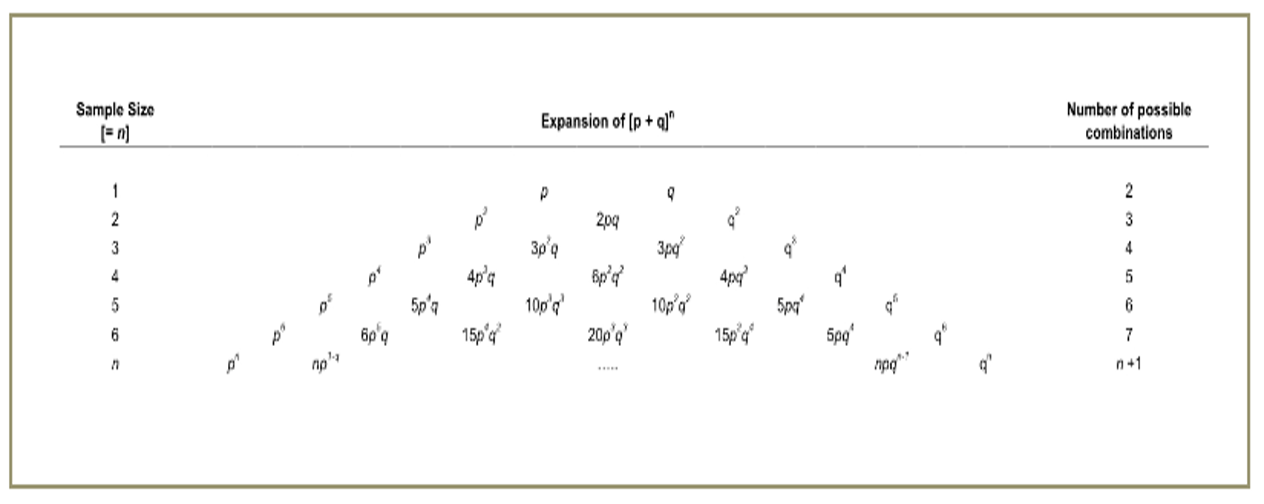
\includegraphics[width=1\linewidth]{1 Introducción/Tareas Capítulo 1/Triángulo de Pascal/Picture3.png}
    \caption{Example: GENETICS}
    \label{fig:enter-label}
\end{figure}

\noindent So - if we look at the family with 3 possible children [n = 3] and if read along the Triangle, we see that for all 3 of the children to have Type I Antithrombin deficiency the probability is [q]3 where q = 1/2 and so [1/2]3 = 1/8. \\
\noindent Antithrombin deficiency is an autosomally inherited disorder and the risk of inheriting a mutant allele from a parent is 1/2 and of not inheriting it, is also 1/2.   So the probability that all 3 children will be normal [p]3 is 1/8 and similarly the probability that all 3 children will have Type 1 Antithrombin deficiency, is [q]3 which is also 1/8. \\
To establish if only 1 of the children will be affected and the other two normal then again we read along from n=3 to where we see 3pq2 and so 3pq2 = 3 x 1/2 x [1/2]2 = 3 x 1/2 x 1/4 = 3/8. So the risk that they will have one affected child and two normal children is 3/8.
\noindent Remember p is the probability of an event not occurring - in this case not inheriting the disorder and q is the probability of an event occurring - in this case inheriting the disorder \\

\noindent Podemos construir el triangulo en python tambien, de la siguiente manera. \\

\begin{verbatim}
    # Doing the Pascal's Triangle using Python
    def factorial(num):
        if num > 0:
            # Doing the factorial using recursion
            return int(num*factorial(num-1))
        else:
            return 1
    
    def combinatoria(num1, num2):
        return int(factorial(num1) / (factorial(num2)*factorial(num1-num2)))
    
    def crearTriangulo(n_filas):
        for fila in range(n_filas):
            for j in range(n_filas-fila+1):
                print(" ", end="")
            if fila == 0:
                print("1 1")
            else:
                for j in range(fila+2):
                    print(combinatoria(fila+1, j), end=" ")
                print()
    
    crearTriangulo(int(input("Indica el número de filas que desee: ")))
    
\end{verbatim}

\noindent O en C++, utilizando en siguiente codigo:\\

\begin{verbatim}
    #include<iostream>
    
    long factorial(int x){
    	if(x > 0){
    		return x * factorial(x-1); //Recursividad
    	}else{
    		return 1;
    	}
    }
    int combinatoria(int num1, int num2){
    	return ((int) factorial(num1))/ (factorial(num2)*factorial(num1-num2));
    }
    void imprimirTriangulo(int filas){
    	for(int i=1;i<=filas;i++){
    		for(int j=0;j<(filas-i);j++){
    			std::cout<<" ";
    		}
    		if(i == 1){
    			std::cout<<"1 1"<<std::endl;
    		}else{
    			for(int j=0;j<=i;j++){
    				std::cout<<combinatoria(i, j)<< " ";
    			}
    			std::cout <<std::endl;
    		}
    	}
    }
    int main(){
    	int filas = 0;
    	std::cout<<"Escribe el número de niveles que desea: "<<std::endl;
    	std::cin >> filas;
    	imprimirTriangulo(filas);
        return 0;
    }
    
\end{verbatim}

%\textbf{References} \\

%1. Knott, R. (2018). Pascal's Triangle. From https://www.mathsisfun.com/pascals-triangle.html \\

%2. Online Mendelian Inheritance in Man, OMIM®. (2021). Johns Hopkins University. Retrieved from https://www.omim.org/ \\

%3. "Principles of Genetics" by D. Peter Snustad and Michael J. Simmons. \\

%4. "Population Genetics: A Concise Guide" by John H. Gillespie. \\

%5. "Population Genetics and Microevolutionary Theory" by Alan R. Templeton. \\

%\begin{center} 
    \newdimen\R
    \R=.4cm
    \def\lim{12} %largo
    \newcommand\mycolor{white}
    \newcommand\thik{\pgflinewidth}
    \begin{tikzpicture}[line width=.2pt]
        \foreach \k in {0,...,\lim}{
        \begin{scope}[shift={(-60:{sqrt(3)*\R*\k})}]
            \pgfmathtruncatemacro\ystart{\lim-\k}
            \foreach \n in {0,...,\ystart}{
            \pgfmathtruncatemacro\newn{\n+\k}
            %binomila ceeficients
            \pgfmathsetmacro{\value}{1};
            \ifthenelse{\k>0}{
            \foreach \b in {1,...,\k}{
            \pgfmathtruncatemacro{\value}{\value*(\newn-\b+1)/\b)};
            \global\let\value=\value
            }
            }{};
            \def\res{3}
            \pgfmathtruncatemacro{\rest}{mod(\value,\res)};
            \ifthenelse{\rest=0}{\def\mycolor{green}}{}
            
            \begin{scope}[shift={(-120:{sqrt(3)*\R*\n})}]
                \draw[top color=\mycolor!20,bottom color=\mycolor!60] 
                (30:\R) \foreach \x in {90,150,...,330} {
                -- (\x:\R)}
                --cycle (90:0) node {\tiny $\mathbf{\value}$};
            \end{scope}
            }
        \end{scope}
        }
    \end{tikzpicture}
\end{center}


\subsubsection{Binomial}
%---------------------------------------------
%                Ejercicio 1
%---------------------------------------------

\noindent \textbf{Ejercicio 1:} Demostrar que

\begin{equation*}
    \binom{n}{k} = \binom{n}{n-k}
\end{equation*}

\noindent \textbf{Solución: } Recordemos que

\begin{equation}
    \binom{n}{k} = \frac{n!}{(n-k)! k!}
    \label{C1: Tarea Binomio de Newton 1}
\end{equation}

\noindent por otro lado

\begin{equation}
    \begin{split}
        \binom{n}{n-k} & = \frac{n!}{(n-(n-k))! (n-k)!} \\
        & = \frac{n!}{k!(n-k)!}
    \end{split}
    \label{C1: Tarea Binomio de Newton 2}
\end{equation}

\noindent Por lo tanto, por (\ref{C1: Tarea Binomio de Newton 1}) y (\ref{C1: Tarea Binomio de Newton 2}):

\begin{equation}
    \binom{n}{k} = \binom{n}{n-k}
\end{equation}

%---------------------------------------------
%                Ejercicio 2
%---------------------------------------------

\noindent \textbf{Ejercicio 2:} Demostrar que

\begin{itemize}
    \item [a) ]
    \begin{equation*}
        \binom{n}{0} = 1
    \end{equation*}

    \item[b) ] 
    \begin{equation*}
        \binom{0}{k} = 0
    \end{equation*}
\end{itemize}

\noindent \textbf{Solución: } 

\begin{itemize}
    \item [a) ]

    \begin{equation*}
        \begin{split}
            \binom{n}{0} & = \frac{n!}{(n)! 0!} \\
            & = \frac{n!}{n!(1)} \\
            & = 1
        \end{split}
    \end{equation*}

    \item [b) ] La expresión $\binom{n}{k}$ se define como el número de formas en que se pueden elegir $k$ elementos de un conjunto de $n$ elementos, pero si $n=0$, no hay elementos en el conjunto, por lo tanto, $\binom{0}{k}$ debe ser igual a cero.
\end{itemize}



\subsubsection{Binomio de Newton}
\noindent \textbf{Binomio de Nexton}.\\
    \noindent Un \textbf{binomio} es un polinomio que consta de dor t\'erminos, como: 
    \begin{center}
        $a+b$, $x^{2}-y$, $\frac{a}{3}-\frac{5mx^{4}}{6b^{2}}$...
    \end{center}
    
    \noindent Existe un procedimiento  para calcular la potencia de un binomio, llamado \textbf{\textit{teorema del binomio de Newton}} o fórmula para el binomio de Newton. Donde para un n\'umero $n$ el desarrollo de:

    \begin{align*}
(a + b)^n &= \binom{n}{0}a^n b^0 + \binom{n}{1}a^{n-1}b^1 + \binom{n}{2}a^{n-2}b^2 + \ldots + \binom{n}{n-1}a^1b^{n-1} + \binom{n}{n}a^0b^n \\
&= a^n + \binom{n}{1}a^{n-1}b + \binom{n}{2}a^{n-2}b^2 + \ldots + \binom{n}{n-1}ab^{n-1} + b^n
\end{align*}\\

    Queda simplificado en:
    \begin{equation}
        (a + b)^n = \sum_{k=0}^{n} \binom{n}{k} a^{n-k} b^k
    \end{equation}\\

\noindent \textit{\textbf{Donde Si $n$ es antural, el desarrollo de $(a+b)^{n}$ cumple con las siguientes caracter\'isticas:}}

\begin{itemize}{}
    \item El primer t\'ermino es $a^{n}$ y el \'ultimo t\'ermino es $b^{n}$.
    \item Al desarrollar el binomio se obitnen $(n+1)$ t\'erminos.
    \item Conforme aumentan los t\'erminos, la potencia del primer t\'ermino $a$ disminuye en 1 y la del segundo t\'ermino aumenta en 1.
    \item Para obtener el i-\'esimo t\'ermino se utiliza la f\'ormula:


    \begin{equation}
        \text{i-\'esimo} = \binom{n}{i} \cdot a^{n-i} \cdot b^i
    \end{equation}
    
    \item Sus coeficientes llamados \textit{coeficientes binomiales}, están dados por la f\'ormula:

    \begin{equation}
        \binom{n}{k} = \frac{n!}{(k!(n-k)!} = \frac{n(n-1)(n-2)\dotsb(n-k+1)}{k!} \\
    \end{equation}

    siendo $n!$ el \textit{factorial} de un n\'umero $n$ natural, el cual se define como

    \begin{center}
         $n! = \begin{cases}
                      1 & \text{si } n = 0 \\
                      n \cdot (n-1)! & \text{si } n \geq 1
                \end{cases}$
    \end{center}

  


\end{itemize}

    
    
\noindent Primeros 10 ejemplos del desarollo del Binomio de Newton: \\

\begin{align*}
    (x + y)^0 & = 1\\  (x + y)^1 & = x + y \\
    (x + y)^2 & = x^2 + 2xy + y^2 \\
    (x + y)^3 & = x^3 + 3x^2y + 3xy^2 + y^3 \\
    (x + y)^4 & = x^4 + 4x^3y + 6x^2y^2 + 4xy^3 + y^4 \\
    (x + y)^5 & = x^5 + 5x^4y + 10x^3y^2 + 10x^2y^3 + 5xy^4 + y^5 \\
    (x + y)^6 & = x^6 + 6x^5y + 15x^4y^2 + 20x^3y^3 + 15x^2y^4 + 6xy^5 + y^6 \\
    (x + y)^7 & = x^7 + 7x^6y + 21x^5y^2 + 35x^4y^3 + 35x^3y^4 + 21x^2y^5 + 7xy^6 + y^7 \\
    (x + y)^8 & = x^8 + 8x^7y + 28x^6y^2 + 56x^5y^3 + 70x^4y^4 + 56x^3y^5 + 28x^2y^6 + 8xy^7 + y^8 \\
    (x + y)^9 & = x^9 + 9x^8y + 36x^7y^2 + 84x^6y^3 + 126x^5y^4 + 126x^4y^5 + 84x^3y^6 + 36x^2y^7 + 9xy^8 + y^9 \\
    (x + y)^{10} & = x^{10} + 10x^9y + 45x^8y^2 + 120x^7y^3 + 210x^6y^4 + 252x^5y^5 + 210x^4y^6 + 120x^3y^7 + 45x^2y^8 + 10xy^9 + y^{10}
\end{align*}   


\subsubsection{Teorema de comletitud de Gödel}
\noindent \textbf{Teorema:} En una lógica de primer orden, toda fórmula que es válida en un sentido lógico es demostrable.\cite{Teorema_de_completitud} \\

\noindent Una lógica de primer orden, también llamada lógica predicativa, lógica de predicados o cálculo de predicados, es un sistema formal diseñado para estudiar la inferencia en los lenguajes de primer orden. Los lenguajes de primer orden son, a su vez, lenguajes formales con cuantificadores que alcanzan solo a variables de individuo, y con predicados y funciones cuyos argumentos son solo constantes o variables de individuo.

\subsubsection{Axioma}
\noindent Los axiomas son afirmaciones que se aceptan como verdaderas y cuya veracidad no puede ser demostrada a partir de otros axiomas.\cite{Definición_de_axioma}

\subsubsection{Paradoja del barbero}
\noindent \textbf{Paradojas y antinomias:} 1. Paradoja: Una paradoja es una declaración o situación que parece llevar a una contradicción lógica o a resultados inesperados y aparentemente contradictorios. \\

\noindent 2. Antinomia: El término "antinomia" no se utiliza comúnmente en el mismo sentido que "paradoja". Sin embargo, en algunos contextos, una antinomia se refiere a una contradicción entre dos afirmaciones o principios que, en teoría, deberían ser mutuamente excluyentes. Una antinomia puede surgir cuando dos reglas o axiomas se contradicen entre sí, lo que plantea un desafío a la consistencia lógica de un sistema o conjunto de creencias. En general, una antinomia se considera un tipo específico de paradoja que involucra principios o reglas en conflicto. \\

\noindent En resumen, una paradoja es una situación que parece llevar a una contradicción lógica o a resultados sorprendentes, mientras que una antinomia es una contradicción entre dos principios o reglas que deberían ser mutuamente excluyentes. Ambos términos se utilizan en el contexto de la lógica, la filosofía y otros campos para describir situaciones que desafían nuestras expectativas racionales. \\

\noindent 1. Paradoja de Russell (también conocida como Paradoja del Conjunto de Todos los Conjuntos que no se Contienen a Sí Mismos): \\

\noindent La Paradoja de Russell se presenta cuando consideramos el conjunto que contiene todos los conjuntos que no se contienen a sí mismos. La pregunta es si este conjunto se contiene a sí mismo o no. Si asumimos que se contiene a sí mismo, entonces no debería incluirse en el conjunto, ya que solo debería contener conjuntos que no se contienen a sí mismos. Por otro lado, si asumimos que no se contiene a sí mismo, entonces debería incluirse en el conjunto, ya que cumple con la condición de no contenerse a sí mismo. Esta paradoja muestra una contradicción en la teoría de conjuntos ingenua y condujo al desarrollo de la teoría de conjuntos axiomática para evitar paradojas como esta. \\

\noindent 2. Antinomia de Cantor: Aunque el término "antinomia" no se usa comúnmente en este contexto, se puede considerar la paradoja de Cantor como un ejemplo de antinomia en la teoría de conjuntos. Georg Cantor demostró que no se puede establecer una correspondencia uno a uno entre el conjunto de todos los números naturales y el conjunto de todos los números reales, lo que implica que hay infinitos de diferentes "tamaños". Sin embargo, esto parece contradecir la intuición de que todos los infinitos son iguales en tamaño. Esta aparente contradicción entre la intuición y el resultado matemático se puede considerar una antinomia en el sentido de que desafía nuestras expectativas comunes. \\

\noindent En resumen, una paradoja es una declaración o situación que parece llevar a una contradicción lógica o a resultados inesperados, como la Paradoja de Russell en la teoría de conjuntos. Por otro lado, una antinomia podría considerarse una contradicción aparente o un conflicto entre la intuición y los resultados matemáticos, como la Antinomia de Cantor en el contexto de los infinitos en la teoría de conjuntos. Ambas destacan la importancia de una formulación cuidadosa de las teorías matemáticas y lógicas. \\

\noindent \textbf{Paradoja del barbero:} En un lejano poblado de un antiguo emirato había un barbero llamado As-Samet diestro en afeitar cabezas y barbas, maestro en escamondar pies y en poner sanguijuelas. Un día el emir se dio cuenta de la falta de barberos en el emirato, y ordenó que los barberos solo afeitaran a aquellas personas que no pudieran afeitarse a sí mismos. ¡Ah! e impuso la norma de que todo el mundo estuviera afeitado, (no se sabe si por higiene, por estética, o por demostrar que podía imponer su santa voluntad y mostrar así su poder). Cierto día el emir llamó a As-Samet para que lo afeitara y él le contó sus angustias:\cite{Paradoja_del_barbero} \\

 \noindent —En mi pueblo soy el único barbero. No puedo afeitar al barbero de mi pueblo, ¡que soy yo!, ya que si lo hago, entonces puedo afeitarme por mí mismo, por lo tanto ¡no debería afeitarme! pues desobedecería vuestra orden. Pero, si por el contrario no me afeito, entonces algún barbero debería afeitarme, ¡pero como yo soy el único barbero de allí!, no puedo hacerlo y también así desobedecería a vos mi señor, oh emir de los creyentes, ¡que Allah os tenga en su gloria!\\

\noindent El emir pensó que sus pensamientos eran tan profundos, que lo premió con la mano de la más hermosa de sus concubinas. Así, el barbero As-Samet vivió para siempre feliz y barbón.


\subsubsection{Paradoja del hotel infinito}

\noindent \textbf{Definición del Problema:}

\noindent Supongamos que tenemos un hotel con un número infinito de habitaciones, numeradas desde $1$ hasta $n$ (donde $n$ es infinito). Además, imaginemos que todas las habitaciones están ocupadas.\\

\noindent Ahora, llega un nuevo huésped al hotel, y nos preguntamos: ¿Podemos acomodar a este nuevo huésped sin rechazar a ninguno de los huéspedes actuales?\\

\noindent \textbf{Solución Sorprendente:} \\

\noindent La solución propuesta por Georg Cantor, el matemático que introdujo esta paradoja, es sorprendente. En lugar de simplemente decir que no hay espacio, Cantor sugirió que podríamos mover a cada huésped actual a la habitación siguiente.\\

\noindent Por ejemplo, el huésped en la habitación $1$ se mueve a la habitación $2$, el huésped en la habitación $2$ se mueve a la habitación $3$, y así sucesivamente. Este proceso se realiza para todas las habitaciones ocupadas. Luego, la habitación $1$ queda libre para el nuevo huésped.\\

\noindent Dado que estamos tratando con un conjunto infinito de habitaciones, siempre habrá una "habitación siguiente" para cada huésped, y podemos hacer espacio para un nuevo huésped de esta manera. \\

\noindent \textbf{Implicaciones Filosóficas y Matemáticas:} \\

\noindent La Paradoja del Hotel Infinito plantea cuestiones profundas sobre la naturaleza del infinito. En un conjunto infinito, las reglas de intuición cotidiana pueden no aplicarse de la misma manera que lo hacen en conjuntos finitos. \\

\noindent Esta paradoja fue un componente clave en el trabajo de Cantor sobre la teoría de conjuntos y los números transfinitos. Cantor demostró que hay diferentes "tamaños" de infinito, y esto cambió fundamentalmente la forma en que los matemáticos piensan sobre el concepto de infinito.\\

\noindent En resumen, la Paradoja del Hotel Infinito es un ejemplo intrigante de cómo los conceptos abstractos en matemáticas, como el infinito, pueden llevar a resultados sorprendentes que desafían nuestra intuición inicial. Además, esta paradoja ha influido en el desarrollo de la teoría de conjuntos y ha tenido implicaciones filosóficas significativas en nuestra comprensión del infinito. \\


\subsubsection{Tipos de infinitos}
\noindent \textbf{Infinitos:} 1. Infinito Contable (\( \aleph_0 \) o Aleph-Cero): Este es el tipo de infinito que se asocia con conjuntos infinitos que tienen una correspondencia uno a uno con los números naturales (\( 1, 2, 3, \ldots \)). Por ejemplo, el conjunto de todos los números naturales es infinito contable.\\

\noindent 2. Infinito No Contable (\( \aleph_1 \) o Aleph-Uno): Estos son conjuntos infinitos que no pueden ponerse en correspondencia uno a uno con los números naturales. El conjunto de todos los números reales es un ejemplo de conjunto infinito no contable. \\

\noindent 3. Infinito más grande (Infinito no enumerable): Cantor demostró que hay infinitos de diferentes "tamaños" y que no podemos enumerar todos los conjuntos infinitos. Por lo tanto, existe un infinito más grande que el infinito contable y el infinito no contable, y este infinito se llama "infinito no enumerable". \\

\noindent 4. Infinito Ordinal: En teoría de conjuntos, se definen números ordinales que representan ciertos tipos de orden entre conjuntos infinitos. Estos ordinales son diferentes de los números cardinales que describen el tamaño de los conjuntos infinitos. Por ejemplo, \( \omega \) (omega) es el primer ordinal infinito y representa la ordenación de los números naturales. \\


\subsubsection{Conjuntos}
\noindent \textbf{Conjunto potencia.} \\
Considerando un \textit{cojunto de conjuntos} tal como $S$, donde $S$ es la clase de todos sus subconjuntos. Se le llama \textbf{conjunto potencia} de $S$ a esta clase de conjuntos y es denotado como $P(S)$. 
Donde su n\'umero de elementos en $P(S)$ es 2 elevado a la potencia de $n(S)$; eso es,

    \begin{center}
        $n(P(S)) = 2 P(S)^{n(S)}$.
    \end{center}

    \textbf{Ejemplo:}
        Suponga $S = \lbrace a,b,c\rbrace$ \\ \vspace{5px}

        Entonces $P(S) = \lbrace \emptyset, \lbrace a\rbrace,  \lbrace b\rbrace,  \lbrace c\rbrace,  \lbrace a, b\rbrace,  \lbrace a, c\rbrace, \lbrace b, c\rbrace, \lbrace a,b,c\rbrace \rbrace$.\\

    Se escribe $P(S) = \{X \,|\, X \subseteq A\}$. Nótese que todos los elementos de $P(S)$ son conjuntos.\\



% Ejemplos
\textbf{Ejemplos:} 
\begin{itemize}
    \item $P(\emptyset) = \{\emptyset\}$.
    \item Si $X = \{a\}$, entonces $P(X) = \{\emptyset, \{a\}\} = \{\emptyset, X\}$.
    \item Si $X = \{\emptyset, \{\emptyset\}, \{a\}, \{b\}, \{\emptyset, a\}, \{\emptyset, b\}, \{a, b\}, X\}$.
\end{itemize}


Como para cada subconjunto $X$, $\emptyset \subseteq X$, entonces $P(X) = \emptyset$ tendrá por lo menos dos elementos que son $\emptyset$ y $X$.

% Teorema 1
\textbf{Teorema 1.} \\
Para cualesquiera conjuntos $A$ y $B$, $$P(A \cup B) \supseteq P(A) \cup P(B).$$

\textbf{Demostración.}Tenemos que 
\begin{align*}
X \in P(A) \cup P(B) &\Rightarrow X \subseteq A \lor X \subseteq B \\
&\Rightarrow X \subseteq A \cup B \\
&\Rightarrow X \in P(A \cup B).
\end{align*}


% Ejemplo que muestra que la otra inclusión no siempre se cumple
\textbf{Ejemplo.} La otra inclusión no siempre se cumple, veamos un ejemplo. Consideremos los conjuntos $A = \{1, 2, 3\}$ y $B = \{2, 3, 4\}$. Tenemos entonces:
\begin{align*}
    P(A) &= \{\emptyset, \{1\}, \{2\}, \{3\}, \{1, 2\}, \{1, 3\}, \{2, 3\}, \{1, 2, 3\}\} \\
    P(B) &= \{\emptyset, \{2\}, \{3\}, \{4\}, \{2, 3\}, \{3, 4\}, \{2, 4\}, \{2, 3, 4\}\}
\end{align*}
Y la unión de los conjuntos potencia es:
\begin{align*}
    P(A) \cup P(B) &= \{\emptyset, \{1\}, \{2\}, \{3\}, \{4\}, \{1, 2\}, \{1, 3\}, \{2, 3\}, \{3, 4\}, \{1, 2, 3\}, \{2, 3, 4\}\}
\end{align*}
Por otro lado, $A \cup B = \{1, 2, 3, 4\}$, de manera que:

%% NO SE CÓMO ACOMODAR ESTO :C
\begin{align}
    P(A \cup B) &= \{\emptyset, \{1\}, \{2\}, \{3\}, \{4\}, \{1, 2\}, \{1, 3\}, \{1, 4\}, \{2, 3\}, \{2, 4\}, \{3, 4\}, \{1, 2, 3\}, \{1, 2, 4\}, \{1, 3, 4\}, \{2, 3, 4\}, \{1, 2, 3, 4\}\}\\
\end{align}
%%%%%%%%%%%%%%%%%%%%%%%%%%%%%%%%%%%%%%%%%%%%%%%%%%%%%%%%%%%%%%%

Observamos que $ \{1, 2, 3, 4\} \subset P(A \cup B)$, y $\{1, 2, 3, 4\} \not\subset P(A) \cup P(B)$. Por lo tanto, la otra inclusión no siempre se cumple.\\

% Teorema 2
\textbf{Teorema 2.}\\ Para cualesquiera conjuntos $A$ y $B$, $$P(A \cap B) = P(A) \cap P(B).$$

\textbf{Demostración.} Tenemos que 
\begin{align*}
X \in P(A) \cap P(B) &\Leftrightarrow X \in P(A) \land X \in P(B) \\
&\Leftrightarrow X \subseteq A \land X \subseteq B \\
&\Leftrightarrow X \subseteq A \cap B \\
&\Leftrightarrow X \in P(A \cap B).
\end{align*}


\vspace{10px} \noindent  \textbf{Conjunto producto.} \\    
 Sean $A$ y $B$ dos conjuntos. El \textit{conjunto producto} de $A$ y $B$, expresado como $A \times B$, est\'a formado por todas las parejas ordenadas $(a,b)$ donde $a \in A$ y $b \in B$:

        \begin{center}
            $A \times B = \lbrace (a,b) : a \in A, b \in B\rbrace$.
        \end{center}

   \textbf{Ejemplo:}  Sea $A = \lbrace a, b \rbrace$, $B = \lbrace 1, 2 \rbrace$ \\

    El conjunto producto de $A \times B = \lbrace(a, 1), (a, 2), (b, 1), (b, 2)\rbrace$. \\
        

    Nota. El producto de un conjunto por sí mismo, $A \times A$, se denota por $A^2$. \vspace{5px}\\
\noindent \textbf{Conjunto producto de $A \times B  \times C.$} \\
         
   \noindent\textbf{Ejemplo:} Sea $A = \lbrace 1, 2 \rbrace$,
    $B = \lbrace x, y, z \rbrace$ y 
    $C = \lbrace 3, 4 \rbrace$.  Encontrar $A \times B  \times C.$ \\

    \noindent$A \times B  \times C$ consta de todos los elementos ordenados de $(a,b,c)$ donde $a \in A$, $b \in B$, $c \in C$. Estos elementos de $A \times B  \times C.$ se pueden obtener sistem\'aticamente mediante el llamado diagrama de \'arbol. \\

    Donde $n(A) = 2$, $n(B) = 3$ y $n(C) = 2$,  por lo que:

    \begin{center}
       $n(A \times B  \times C) = 12 = n(A) \cdot n(B) \cdot n(C)$
    \end{center}

     \vspace{10px}
     
\begin{multicols}{3}

    \begin{tikzpicture}[level distance=2cm,
      level 1/.style={sibling distance=3cm},
      level 2/.style={sibling distance=1cm},
      level 3/.style={sibling distance=0.5cm},grow=right]
  
      \node {$A \times B \times C$}
        child { node {$1$}
              child { node {$x$}
                child {
                  node {$3$}
                }
                child {
                  node {$4$}
                }
              }
              child { node {$y$}
                child {
                  node {$3$}
                }
                child {
                  node {$4$}
                }
              }
              child {   node {$z$}
                child {
                  node {$3$}
                }
                child {
                  node {$4$}
                }
              }
        }
        child {  node {$2$}
          child {    node {$x$}
            child {
              node {$3$}
            }
            child {
              node {$4$}
            }
          }
          child {  node {$y$}
            child {
              node {$3$}
            }
            child {
              node {$4$}
            }
          }
          child {    node {$z$}
            child {
              node {$3$}
            }
            child {
              node {$4$}
            }
          }
        };
    
    \end{tikzpicture}
        
    \columnbreak
    \hspace{1cm}
    \columnbreak
    
    \begin{itemize}
     \renewcommand\labelitemi{}
        \item $(2,z,4)$
        \item $(2,z,3)$
        \item $(2,y,4)$
        \item $(2,y,3)$
        \item $(2,x,4)$
        \item $(2,x,3)$
                 
        \item $(1,z,4)$
        \item $(1,z,3)$
        \item $(1,y,4)$
        \item $(1,y,3)$
        \item $(1,x,4)$
        \item $(1,x,3)$
     \end{itemize}
        
\end{multicols}
        


\\ 

\vspace{10px}\noindent \textbf{Conjuntos Autocontenidos.} \\ Un conjunto se considera \textit{autocontenido} cuando todos sus elementos también son elementos de otro conjunto más grande, es decir, cuando está completamente contenido dentro de otro conjunto.

\noindent \textbf{Definición.}

\noindent Formalmente, un conjunto $A$ se llama autocontenido si para todo elemento $x$ en $A$, $x$ también es un elemento de otro conjunto $B$.

\[
A \subseteq B \quad \text{o} \quad B \supseteq A
\]

\noindent Esto significa que $A$ es un subconjunto de $B$, o equivalentemente, $B$ es un superconjunto de $A$.

\noindent \textbf{Ejemplos:}

\begin{enumerate}
  \item Si consideramos los conjuntos $A = \{1, 2\}$ y $B = \{1, 2, 3, 4\}$, entonces $A$ es un subconjunto de $B$, es decir, $A \subseteq B$, porque todos los elementos de $A$ (1 y 2) también están en $B$.
  
  \item Tomemos los conjuntos $C = \{a, b, c\}$ y $D = \{a, b, c, d, e\}$. En este caso, $C$ es un subconjunto de $D$ ya que todos los elementos de $C$ (a, b y c) también están en $D$.
  
  \item Si consideramos el conjunto vacío $\emptyset$, este conjunto es un subconjunto de cualquier otro conjunto. Por ejemplo, $\emptyset \subseteq A$ para cualquier conjunto $A$, ya que no contiene ningún elemento que no esté en $A$.
\end{enumerate}

\subsubsection{Tensor de Levi-Civita}
\textbf{Tensor de Levi-Civita:} El tensor de Levi-Civita, denotado comúnmente como $$ \varepsilon_{ijk} $$, es una estructura tensorial fundamental en el contexto de espacios tridimensionales. Se utiliza para describir propiedades de orientación, simetría y cálculos vectoriales en un espacio euclidiano tridimensional (como el espacio 3D que experimentamos en el mundo real). \\

Definición de Componentes: Las componentes del tensor de Levi-Civita se definen de la siguiente manera: \\

\begin{equation}
\varepsilon_{ijk} es igual a 1 si los índices (i, j, k) forman una permutación par de (1, 2, 3).
\end{equation}
Por ejemplo, 
\begin{equation}
\varepsilon_{123} = \varepsilon_{231} = \varepsilon_{312} = 1.
\end{equation}
\begin{equation}
\varepsilon_{ijk} es igual a -1 si los índices (i, j, k) 
\end{equation}

forman una permutación impar de (1, 2, 3). 

Por ejemplo, 
\begin{equation}
\varepsilon_{213} = \varepsilon_{132} = \varepsilon_{321} = -1.
\end{equation}

\begin{equation}
\varepsilon_{ijk} es igual a 0 si hay índices repetidos en la permutación. 
\end{equation}
Por ejemplo, 
\begin{equation}
\varepsilon_{112} = \varepsilon_{122} = \varepsilon_{222} = 0.
\end{equation}

\textbf{Propiedades y Aplicaciones:} \\

\textbf{Producto Cruz:} El tensor de Levi-Civita se utiliza para definir el producto cruz de dos vectores en matemáticas y física. Si tienes dos vectores A y B, su producto cruz A × B se expresa utilizando las componentes del tensor de Levi-Civita.\\

\textbf{Regla de la Mano Derecha:} El tensor de Levi-Civita se relaciona con la regla de la mano derecha, que es fundamental en mecánica y electromagnetismo. Esta regla se utiliza para determinar la dirección de un vector resultante cuando se cruzan dos vectores.

\textbf{Teoría del Campo Electromagnético:} En electromagnetismo, el tensor de Levi-Civita se usa en la expresión de la Ley de Biot-Savart y en la Ley de Ampère para describir campos magnéticos generados por corrientes eléctricas.

\textbf{Teoría de la Relatividad General:} En la teoría de la relatividad general de Einstein, el tensor de Levi-Civita se utiliza para definir la métrica espacio-temporal y las ecuaciones de campo de Einstein, que describen la curvatura del espacio-tiempo debido a la presencia de masa y energía.

\textbf{Mecánica de Sólidos y Fluidos:} En la mecánica de materiales, el tensor de Levi-Civita se utiliza en la teoría de elasticidad y en la descripción de deformaciones en sólidos y fluidos.

\textbf{Geometría Diferencial:} En geometría diferencial, el tensor de Levi-Civita se utiliza para definir la conexión de Levi-Civita, que es fundamental en la teoría de la relatividad y la geometría riemanniana.  \clearpage

\subsubsection{Traducción de artículos}
\section*{Los primates cuentan}

\noindent Hace alrededor de 60 millones de años, pequeños primates parecidos a lémures habían evolucionado en diversas partes del mundo, y hace 30 millones de años ya existían primates con características similares a los monos. ¿Podían contar tales criaturas? El significado del conteo por parte de los animales es un tema altamente controvertido entre los expertos en comportamiento animal. Sin embargo, muchos académicos sugieren que los animales tienen algún sentido del número. H. Kalmus escribe en su artículo "Animals as Mathematicians" publicado en la revista Nature: \\

\begin{quote}
  No hay duda de que algunos animales, como las ardillas o los loros, pueden ser entrenados para contar. ... Se han informado facultades de conteo en ardillas, ratas y para insectos polinizadores. Algunos de estos animales y otros pueden distinguir números en patrones visuales de lo contrario similares, mientras que otros pueden ser entrenados para reconocer e incluso reproducir secuencias de señales acústicas. Incluso algunos pueden ser entrenados para golpear el número de elementos (puntos) en un patrón visual.... La falta del numeral hablado y el símbolo escrito hace que a muchas personas les cueste aceptar a los animales como matemáticos.
\end{quote}

\noindent Se ha demostrado que las ratas "cuentan" al realizar una actividad el número correcto de veces a cambio de una recompensa. Los chimpancés pueden presionar números en una computadora que coinciden con la cantidad de plátanos en una caja. Testsuro Matsuzawa, del Instituto de Investigación de Primates de la Universidad de Kyoto en Japón, enseñó a un chimpancé a identificar números del 1 al 6 presionando la tecla de la computadora correspondiente cuando se le mostraba una cierta cantidad de objetos en la pantalla de la computadora. \\

\noindent Michael Beran, científico investigador en la Universidad Estatal de Georgia en Atlanta, Georgia, entrenó a chimpancés para usar una pantalla de computadora y un joystick. La pantalla mostraba un número y luego una serie de puntos, y los chimpancés tenían que hacer coincidir ambos. Un chimpancé aprendió los números del 1 al 7, mientras que otro logró contar hasta 6. Cuando los chimpancés fueron probados nuevamente después de tres años, ambos pudieron igualar los números, pero con el doble de la tasa de error.
 \clearpage

\section*{Números primos generados por cígarras}

\noindent Las cícadas son insectos alados que evolucionaron alrededor de hace 1.8 millones de años durante el Pleistoceno, cuando los glaciares avanzaron y retrocedieron a lo largo de América del Norte. Las cícadas del género Magicicada pasan la mayor parte de sus vidas bajo tierra, alimentándose de los jugos de las raíces de las plantas, para luego emerger, aparearse y morir rápidamente. \\ 

\noindent Estas criaturas muestran un comportamiento sorprendente: su emergencia está sincronizada con períodos de años que suelen ser números primos, como 13 y 17. (Un número primo es un entero como 11, 13 y 17 que tiene solo dos divisores enteros: 1 y él mismo). Durante la primavera de su año 13º o 17º, estas cícadas periódicas construyen un túnel de salida. \\

\noindent A veces, más de 1.5 millones de individuos emergen en un solo acre; esta abundancia de cuerpos puede tener valor de supervivencia al abrumar a depredadores como pájaros que no pueden posiblemente comerlos todos de una vez.
Algunos investigadores han especulado que la evolución de ciclos de vida de números primos ocurrió para que las criaturas aumentaran sus posibilidades de evadir a depredadores y parásitos de vida más corta. Por ejemplo, si estas cícadas tuvieran ciclos de vida de 12 años, todos los depredadores con ciclos de vida de 2, 3, 4 o 6 años podrían encontrar más fácilmente a los insectos. Mario Markus del Instituto Max Planck de Fisiología Molecular en Dortmund, Alemania, y sus colegas descubrieron que este tipo de ciclos de números primos surgen naturalmente a partir de modelos matemáticos evolutivos de interacciones entre depredador y presa. Para experimentar, asignaron primero duraciones de ciclo de vida aleatorias a sus poblaciones simuladas por computadora. Después de algún tiempo, una secuencia de mutaciones siempre bloqueaba a las cícadas sintéticas en un ciclo de números primos estable. \\

 \clearpage
%\noindent \textbf{Ant Odometer}
\section*{Ant odometer}

\noindent Las hormigas son insectos sociales que evolucionaron a partir de avispas vespoideas a mediados del período Cretácico, hace unos 150 millones de años. Tras el surgimiento de las plantas con flores, hace unos 100 millones de años, las hormigas se diversificaron en numerosas especies.\\

\noindent La hormiga del desierto del Sahara, Cataglyphis fortis, recorre inmensas distancias sobre terreno arenoso, a menudo completamente desprovisto de puntos de referencia, en busca de alimento. Estas criaturas pueden regresar a su nido utilizando una ruta directa en lugar de volver sobre su camino de salida. No sólo juzgan direcciones, usando la luz del cielo como orientación, sino que también parecen tener una "computadora" incorporada que funciona como un podómetro que cuenta sus pasos y les permite medir distancias exactas. Una hormiga puede viajar hasta 50 metros hasta que encuentra un insecto muerto, después de lo cual arranca un trozo para llevarlo directamente a su nido, al que se accede a través de un agujero que a menudo tiene menos de un milímetro de diámetro.\\

\noindent Al manipular la longitud de las patas de las hormigas para darles zancadas más largas y más cortas, un equipo de investigación de científicos alemanes y suizos descubrió que las hormigas "cuentan" los pasos para juzgar la distancia. Por ejemplo, una vez que las hormigas llegaron a su destino, las patas se alargaron añadiendo zancos o se acortaron mediante una amputación parcial. Luego, los investigadores devolvieron las hormigas para que pudieran comenzar su viaje de regreso al nido. Las hormigas con zancos viajaron demasiado lejos y pasaron la entrada del nido, mientras que las que tenían las patas amputadas no llegaron. Sin embargo, si las hormigas comenzaron su viaje desde su nido con las patas modificadas, pudieron calcular las distancias apropiadas. Esto sugiere que la longitud de la zancada es el factor crucial. Además, el cerebro de la hormiga le permite calcular una cantidad relacionada con la proyección horizontal de su camino para que no se pierda incluso si el paisaje arenoso cambia durante su viaje. \clearpage
\section*{Quipu}

\noindent Los antiguos incas usaban quipus, bancos de memoria hechos de cuerdas y nudos, para almacenar números. Hasta hace poco, los quipus más antiguos conocidos databan alrededor del año 650 d.C. Sin embargo, en 2005, un quipu de la ciudad costera peruana de Caral fue fechado hace aproximadamente 5,000 años.\\

\noindent Los incas de América del Sur tenían una civilización compleja con una religión estatal común y un idioma común. Aunque no tenían escritura, mantenían registros extensos codificados por un sistema lógico-numérico en los quipus, que variaban en complejidad desde tres hasta alrededor de mil cuerdas. Desafortunadamente, cuando los españoles llegaron a América del Sur, vieron los extraños quipus y pensaron que eran obras del diablo. Los españoles destruyeron miles de ellos en nombre de Dios, y hoy en día solo quedan alrededor de 600 quipus. \\

\noindent Los tipos y posiciones de nudos, las direcciones de las cuerdas, los niveles de las cuerdas, y el color y el espaciado representan números mapeados a objetos del mundo real. Se utilizaron diferentes grupos de nudos para diferentes potencias de 10. Probablemente, los nudos se utilizaron para registrar recursos humanos y materiales e información del calendario. Los quipus podrían haber contenido más información, como planes de construcción, patrones de danza e incluso aspectos de la historia inca. El quipu desmiente la noción de que las matemáticas florecen solo después de que una civilización ha desarrollado la escritura; sin embargo, las sociedades pueden alcanzar estados avanzados sin haber desarrollado registros escritos. Curiosamente, hoy en día existen sistemas informáticos cuyos gestores de archivos se llaman quipus, en honor a este antiguo dispositivo muy útil. \\

\noindent Una aplicación siniestra del quipu por los incas era como un calculador de muerte. Cuotas anuales de adultos y niños eran ritualmente sacrificadas, y esta empresa se planeaba utilizando un quipu. Algunos quipus representaban al imperio, y las cuerdas se referían a caminos y los nudos a víctimas sacrificiales.
 \clearpage
\section*{Cuadrados mágicos}

\noindent Se sugiere que los cuadrados mágicos se originaron en China y fueron mencionados por primera vez en un manuscrito de la época del Emperador Yu, alrededor del 2200 a.C. Un cuadrado mágico consta de $N^2$ cajas, llamadas celdas, llenas de enteros que son todos diferentes. Las sumas de los números en las filas horizontales, columnas verticales y diagonales principales son todas iguales. \\

\noindent Si los enteros en un cuadrado mágico son los números consecutivos del 1 al $N^2$, se dice que el cuadrado es de orden $N$, y el número mágico, o suma de cada fila, es una constante igual a $\frac{N(N^2 + 1)}{2}$. El artista renacentista Albrecht Dürer creó este maravilloso cuadrado mágico de $4 \times 4$ en 1514. \\

\[
\begin{array}{|c|c|c|c|}
\hline
16 & 13 & 3 & 2 \\
\hline
5 & 10 & 11 & 8 \\
\hline
9 & 6 & 7 & 12 \\
\hline
4 & 15 & 14 & 1 \\
\hline
\end{array}
\]

\noindent Observa que los dos números centrales en la fila inferior leen "1514", el año de su construcción. Las filas, columnas y diagonales principales suman 34. Además, 34 es la suma de los números de las esquinas (16 + 13 + 4 + 1) y del cuadrado central $2 \times 2$ (10 + 11 + 6 + 7). \\

\noindent Tan temprano como en 1693, los 880 diferentes cuadrados mágicos de cuarto orden fueron publicados póstumamente en \textit{Des quassez ou tables magiques} por Bernard Frenicle de Bessy, un destacado aficionado matemático francés y uno de los principales investigadores de cuadrados mágicos de todos los tiempos. \\

\noindent Hemos llegado muy lejos desde los más simples cuadrados mágicos de $3 \times 3$ venerados por civilizaciones de casi todos los períodos y continentes, desde los indios mayas hasta el pueblo Hasua de África. Hoy en día, los matemáticos estudian estos objetos mágicos en dimensiones altas, por ejemplo, en forma de hipercubos de cuatro dimensiones que tienen sumas mágicas en todas las direcciones apropiadas.
 \clearpage

\subsubsection{Paradigmas para calcular el factorial}
 \noindent El cálculo del factorial (n!) es un problema clásico que se puede abordar desde varios paradigmas de programación. Aquí te presento cinco ejemplos, cada uno representando un paradigma diferente:

\noindent 1.Paradigma Imperativo (Procedural)
   En este enfoque, se utiliza un bucle para iterar desde 1 hasta n multiplicando los números.

   python
   \begin{verbatim}
       def factorial_iterativo(n):
           resultado = 1
           for i in range(1, n + 1):
               resultado *= i
           return resultado
  \end{verbatim}

\noindent 2.Paradigma Funcional:
   En programación funcional, se pueden usar funciones recursivas para expresar el cálculo factorial.

   python
   \begin{verbatim}
       def factorial_recursivo(n):
           return 1 if n == 0 else n * factorial_recursivo(n - 1)
   \end{verbatim}

\noindent 3.Paradigma Orientado a Objetos:
   Puedes encapsular el cálculo del factorial dentro de una clase.

   python
   \begin{verbatim}
       class Factorial:
           @staticmethod
           def calcular_factorial(n):
               return 1 if n == 0 else n * Factorial.calcular_factorial(n - 1)
   \end{verbatim}

\noindent 4.Programación Declarativa:
   Enfoque en declarar qué se quiere lograr en lugar de cómo hacerlo. En Python, puedes usar la función `reduce` de la biblioteca `functools`.

   python
   \begin{verbatim}
       from functools import reduce
    
       def factorial_declarativo(n):
           return reduce(lambda x, y: x * y, range(1, n + 1), 1)
   \end{verbatim}

\noindent 5. Programación Lógica:
   Usando lógica y reglas de inferencia, se puede expresar el cálculo del factorial en lenguajes de programación lógica como Prolog.

   prolog
   \begin{verbatim}
       factorial(0, 1).
       factorial(N, F) :- N > 0, N1 is N - 1, factorial(N1, F1), F is N * F1.
   \end{verbatim}

\noindent 6. Programación Concurrente:
   Utilizando hilos o procesos concurrentes para calcular partes del factorial de manera simultánea.

   python
   \begin{verbatim}
       from concurrent.futures import ThreadPoolExecutor
    
       def calcular_factorial_concurrente(n):
           def parcial_factorial(i):
               resultado_parcial = 1
               for j in range(1, i + 1):
                   resultado_parcial *= j
               return resultado_parcial
    
           with ThreadPoolExecutor() as executor:
               resultados_parciales = list(executor.map(parcial_factorial, range(1, n + 1)))
    
           return functools.reduce(lambda x, y: x * y, resultados_parciales, 1)
   \end{verbatim}

\noindent 7. Programación Reactiva:
   Utilizando un enfoque reactivo donde se observan eventos y se actualiza el resultado del factorial en consecuencia.

   python
   \begin{verbatim}
       from rx import Observable
    
       def calcular_factorial_reactivo(n):
           return Observable.range(1, n).scan(lambda acc, x: acc * x).last()
   \end{verbatim}

\noindent 8. Programación Basada en Reglas:
   Utilizando un sistema basado en reglas donde se definen reglas para inferir el resultado del factorial.

   python
   \begin{verbatim}
       from pyknow import KnowledgeEngine
    
       class FactorialEngine(KnowledgeEngine):
           @Rule()
           def base_case(self):
               self.declare(Fact(n=0, factorial=1))
    
           @Rule(Fact(n=MATCH.n), NOT(Fact(factorial=W())))
           def calcular_factorial(self, n):
               self.declare(Fact(n=n, factorial=n * self.factorial(n - 1)))
    
       def calcular_factorial_reglas(n):
           engine = FactorialEngine()
           engine.reset()
           engine.declare(Fact(n=n))
           engine.run()
           return engine.facts[-1].factorial
   \end{verbatim}

\noindent9. Programación Cuántica:
   Solo como curiosidad, podrías explorar implementaciones cuánticas de algoritmos, como el algoritmo cuántico de Shor para factorización.



\subsubsection{Recursividad}

\noindent La recursión es un concepto en programación y matemáticas que implica la definición o descripción de algo en términos de sí mismo. En otras palabras, un problema recursivo puede dividirse en subproblemas más pequeños del mismo tipo. Un procedimiento o función recursiva es aquella que se llama a sí misma para resolver instancias más pequeñas del mismo problema. \\

\noindent La idea fundamental de la recursión es dividir un problema en casos más pequeños y más manejables hasta llegar a un caso base, que es un problema lo suficientemente simple como para resolverse directamente. La solución a los problemas más pequeños se combina de alguna manera para obtener la solución al problema original. \\

\noindent  Ejemplo simple de una función recursiva en programación (usando Python):\\

\begin{verbatim}
    def factorial(n):
        # Caso base
        if n == 0 or n == 1:
            return 1
        else:
            # Llamada recursiva
            return n * factorial(n - 1)
    
    # Ejemplo de uso
    result = factorial(5)
    print(result)  # Salida: 120

\end{verbatim}

\noindent En este ejemplo, la función factorial se define en términos de sí misma. El caso base es cuando n es 0 o 1, en cuyo caso la función devuelve 1. Para valores mayores de n, la función se llama a sí misma con un argumento más pequeño (n - 1). La llamada recursiva continúa hasta que se alcanza el caso base, y luego las soluciones se combinan para obtener el resultado final. \\

\noindent La recursión se utiliza comúnmente en algoritmos y estructuras de datos, y puede ser una forma elegante y poderosa de abordar ciertos problemas. Sin embargo, es importante manejarla cuidadosamente para evitar casos de recursión infinita y asegurarse de que siempre se alcance el caso base. \\



\subsubsection{Moleculas Cis y trans}

\noindent \textbf{Introducción:}\\

\noindent Las moléculas cis y trans son conceptos utilizados para describir la disposición espacial de grupos funcionales alrededor de átomos de carbono en moléculas orgánicas. Estos términos son comúnmente asociados con los isómeros geométricos, que son compuestos con la misma fórmula molecular pero con diferentes arreglos tridimensionales de sus átomos.\\

\noindent \textbf{Definición:}\\

\begin{itemize}
  \item \textbf{Molécula Cis:} En una molécula cis, los grupos iguales o sustituyentes similares están en el mismo lado del doble enlace o anillo. Esto significa que los átomos o grupos unidos a los carbonos de un doble enlace están en el mismo lado del plano de la molécula.

  \item \textbf{Molécula Trans:} En una molécula trans, los grupos iguales o sustituyentes similares están en lados opuestos del doble enlace o anillo. Los átomos o grupos unidos a los carbonos de un doble enlace están en lados opuestos del plano de la molécula.
\end{itemize}

\noindent \textbf{Ejemplos:}\\

\noindent Consideremos el ejemplo de un ácido graso insaturado con un doble enlace:\\

\begin{itemize}
  \item \textbf{Ácido Oleico (Cis):} El ácido oleico es un ácido graso común con un doble enlace cis. En este caso, los dos átomos de hidrógeno en los carbonos del doble enlace están en el mismo lado del plano de la molécula.

  \item \textbf{Ácido Eláico (Trans):} El ácido eláico es otro ácido graso con un doble enlace, pero en este caso, los dos átomos de hidrógeno en los carbonos del doble enlace están en lados opuestos del plano de la molécula.
\end{itemize}

\noindent \textbf{Importancia Biológica:} \\

\noindent La disposición de los grupos en moléculas cis y trans puede afectar significativamente las propiedades físicas y biológicas de los compuestos. Por ejemplo, los ácidos grasos trans se han asociado con efectos adversos para la salud cuando se consumen en exceso, mientras que los ácidos grasos cis son más comunes en los lípidos biológicos.\\

\noindent \textbf{Conclusión:} \\

\noindent En resumen, los conceptos de moléculas cis y trans son esenciales para comprender la geometría molecular y las propiedades de los compuestos orgánicos. La disposición espacial de los grupos alrededor de los dobles enlaces o anillos puede tener implicaciones significativas en la función biológica y en las propiedades físicas de las moléculas. \\




\subsubsection{Congruencia Zeller}
\noindent La Congruencia de Zeller es una fórmula matemática que se utiliza para calcular el día de la semana correspondiente a una fecha específica. Esta fórmula fue desarrollada por Christian Zeller en el siglo XIX. La fórmula toma en cuenta el día, el mes y el año de la fecha y devuelve un número que representa el día de la semana, donde 0 representa el sábado, 1 el domingo, 2 el lunes, y así sucesivamente.

\noindent La fórmula de congruencia de Zeller se define de la siguiente manera:

\begin{equation*}
	h = (q + 13*(m+1)/5 + K + K/4 + J/4 + 5*J) \; mod \; 7
\end{equation*}


\noindent Donde:

\begin{itemize}
	\item h es el día de la semana (0 = sábado, 1 = domingo, 2 = lunes, ..., 6 = viernes).
	
	\item q es el día del mes.
	
	\item m es el mes (3 = marzo, 4 = abril, ..., 12 = diciembre, enero y febrero se cuentan como 13 y 14 del año anterior).
	
	\item K es el año del siglo (el año sin los dos dígitos finales).
	
	\item J es el siglo (los dos primeros dígitos del año).
\end{itemize}

\begin{lstlisting}
	def zeller_congruence(day, month, year):
		# Ajuste del mes y el año para la fórmula de Zeller
		if month in (1, 2):
			month += 12
			year -= 1
	
		# Aplicación de la fórmula de Zeller
		K = year % 100
		J = year // 100
		day_of_week = (day + 13 * (month + 1) // 5 + K + K // 4 + J // 4 - 2 * J) % 7
	
		# Días de la semana
		days = ["Sábado", "Domingo", "Lunes", "Martes", "Miércoles", "Jueves", "Viernes"]
	
		return days[day_of_week]
	
	# Ingresa la fecha en formato DD, MM, YYYY
	day = int(input("Ingresa el día (1-31): "))
	month = int(input("Ingresa el mes (1-12): "))
	year = int(input("Ingresa el año (YYYY): "))
	
	day_of_week = zeller_congruence(day, month, year)
	print(f"El día de la semana es: {day_of_week}")
	
	
\end{lstlisting}

%---------------------------------------------
%                 Bibliografía
%---------------------------------------------
\clearpage
\printbibliography

\end{document}
